\documentclass{article}[11pt]

\usepackage{amsmath}
\usepackage{amssymb}
\usepackage{nicefrac}

\usepackage{pdflscape}

\usepackage{upgreek}

\usepackage{bashful}

% No intendation
\setlength\parindent{0pt}

\usepackage{hyperref}

\usepackage{siunitx}
\sisetup{
  per-mode=fraction,
  fraction-function=\tfrac
}

\usepackage{listings}
  \lstset{
    basicstyle=\ttfamily,
    escapeinside=||,
    xleftmargin=1cm
  }

\usepackage{float}

\usepackage{longtable}

\usepackage{multirow}

\usepackage{tikz}
  \usetikzlibrary{patterns}
  \usetikzlibrary{arrows.meta}
  \usetikzlibrary{shapes.misc}
  \usetikzlibrary{calc}

\usepackage{pgfplots}

\usepackage{cleveref}
\crefmultiformat{equation}{(#2#1#3)}{ and~(#2#1#3)}{, (#2#1#3)}{ and~(#2#1#3)}


\usepackage{acronym}
\usepackage[acronym,nonumberlist]{glossaries}
\glsdisablehyper
\makeglossaries
\newacronym{spice}{SPICE}{Simulation Program with Integrated Circuit Emphasis}
\newacronym{lef}{LEF}{Library Exchange Format}
\newacronym{dft}{DFT}{Discrete Fourier Transform}
\newacronym{dtft}{DTFT}{Discrete-Time Fourier Transform}
\newacronym{fft}{FFT}{Fast Fourier Transform}
\newacronym{mosfet}{MOSFET}{Metal–Oxide–Semiconductor Field-Effect Transistor}
\newacronym{clm}{CLM}{Channel Length Modulation}
\newacronym{de}{DE}{differential equation}
\newacronym{soi}{SOI}{silicon-on-insulator}
\newacronym{ldo}{LDO}{low-dropout regulator}
\newacronym{ota}{OTA}{operational-transconductance amplifier}
\newacronym{ofa}{OFA}{operational-floating amplifier}

% literature
\usepackage[ backend=biber
           , isbn=true
           , sorting=none
           , style=ieee
           ]{biblatex}
\addbibresource{./../../literature.bib}

% definitions
\def \whatis       {Notes}
\def \title        {Fuubar}

\def \author       {Matthias Schweikardt}

\def \authorMail   {mschweikardt@posteo.de}

\def \authorGithub {mschweikardt}

\def \license      {CC BY-SA 4.0}
\def \licenseUrl   {https://creativecommons.org/licenses/by-sa/4.0/}

\def \date         {nodate}

\def \pdfurl       {https://mschweikardt.github.io/ee-notes/%
\bash[stdout]
IFS=/ 
var=($PWD)
echo ${var[-1]}
\END%
.pdf
}
\def \srcurl       {srcurl}


% Customize footer and header of document
\usepackage{fancyhdr}

% Access last page number
\usepackage{lastpage}

% Access last page number
\usepackage[thinc]{esdiff}

% Physics
\usepackage{physics}

% Comment environment
\usepackage{comment}

% Subcaptions
\usepackage{subcaption}

% Thicker lines in tables
\usepackage{booktabs}

% Indentation in footnote
\makeatletter
\renewcommand\@makefntext[1]{\leftskip=2em\hskip-0.5em\@makefnmark#1}
\makeatother         

% qty with the siunitx definition
\AtBeginDocument{\RenewCommandCopy\qty\SI}

% TikZ compatibility
\pgfplotsset{compat=1.18}


\makeatletter
\pgfmathdeclarefunction{myatan2}{2}{%
\begingroup%
  \pgfmathfloattofixed{#1}\edef\tempa{\pgfmathresult}%
  \pgfmathfloattofixed{#2}%
  \pgfkeys{pgf/fpu=false}%
  \pgfmathparse{atan2(\tempa,\pgfmathresult)}\pgfkeys{/pgf/fpu}%
  \pgfmathfloatparsenumber{\pgfmathresult}%
  \pgfmath@smuggleone\pgfmathresult%
\endgroup
}
\makeatother

\usepackage{tabularx}
% usepackages
\usepackage[ a4paper
           , textwidth  = 16.0cm
           , textheight = 25.0cm
           , headsep    =  0.25cm
           , voffset    =  0.3cm
           , footskip   =  1.25cm
           ]{geometry}

% Section and subsection enumeration
\renewcommand{\thesection}{\Roman{section}.} 
\renewcommand{\thesubsection}{\thesection\Alph{subsection}}

\usepackage{titlesec}
\titleformat{\section}
  {\normalfont\Large\bfseries}{\thesection}{0.2em}{}
\titleformat{\subsection}
  {\normalfont\large\bfseries}{\thesubsection}{0.2em}{}


% Defince title of document
\newcommand{\notetitle}{
  \begingroup
  \hypersetup{hidelinks}
  \thispagestyle{notefirst}
  \begin{center}
  \rule{\textwidth}{1pt}\\
  \medskip
  {\it \whatis}\\
  \bigskip
  {\LARGE \textbf{\title}}\\
  \medskip
  {\small \author}\\
  \rule{\textwidth}{0.5pt}\\
  {\small
    \begin{minipage}[t]{0.5\textwidth}
      \begin{tabular}[t]{ p{2.25cm} p{5.75cm}}
        Mail: & \href{mailto:\authorMail}{\tt{\authorMail}} \\
        Github: & \href{https://github.com/\authorGithub}{\tt{\authorGithub}} \\
      \end{tabular}
    \end{minipage}%
    %
    \begin{minipage}[t]{0.5\textwidth}
      \begin{tabular}[t]{ p{2.25cm} p{5.75cm} }
        Date: & \date  \\
        License: & \href{\licenseUrl}{\license}
      \end{tabular}
    \end{minipage}
  }%
  {\small
    \begin{minipage}[t]{\textwidth}
      \begin{tabular}[t]{ p{2.25cm} p{12cm}}
        Latest PDF: & \href{\pdfurl}{\tt{\pdfurl}} \\
        Latest Source: & \href{\srcurl}{\tt{\srcurl}}
      \end{tabular}
    \end{minipage}%
  }
  \bigskip
  \rule{\textwidth}{1pt}
  \end{center}
  \endgroup
}

% Header and footer on first page
\fancypagestyle{notefirst}{
  \fancyhf{}
  \renewcommand{\headrulewidth}{0pt}
  \renewcommand{\footrulewidth}{0pt}

  \fancyfoot[C]{\thepage/\pageref*{LastPage}}
}

% Header and footer on 2nd-last page
\fancypagestyle{noterest}{
  \fancyhf{}
  \renewcommand{\headrulewidth}{0.5pt}
  \renewcommand{\footrulewidth}{0.0pt}

  \fancyhead[L]{\author}
  \fancyhead[C]{\title}
  \fancyhead[R]{\date}

  \fancyfoot[C]{\thepage/\pageref*{LastPage}}
}
\pagestyle{noterest}

\usepackage{amsmath}
\usepackage{amssymb}
\usepackage{nicefrac}

\usepackage{pdflscape}

\usepackage{upgreek}

\usepackage{bashful}

% No intendation
\setlength\parindent{0pt}

\usepackage{hyperref}

\usepackage{siunitx}
\sisetup{
  per-mode=fraction,
  fraction-function=\tfrac
}

\usepackage{listings}
  \lstset{
    basicstyle=\ttfamily,
    escapeinside=||,
    xleftmargin=1cm
  }

\usepackage{float}

\usepackage{longtable}

\usepackage{multirow}

\usepackage{tikz}
  \usetikzlibrary{patterns}
  \usetikzlibrary{arrows.meta}
  \usetikzlibrary{shapes.misc}
  \usetikzlibrary{calc}

\usepackage{pgfplots}

\usepackage{cleveref}
\crefmultiformat{equation}{(#2#1#3)}{ and~(#2#1#3)}{, (#2#1#3)}{ and~(#2#1#3)}


\usepackage{acronym}
\usepackage[acronym,nonumberlist]{glossaries}
\glsdisablehyper
\makeglossaries
\newacronym{spice}{SPICE}{Simulation Program with Integrated Circuit Emphasis}
\newacronym{lef}{LEF}{Library Exchange Format}
\newacronym{dft}{DFT}{Discrete Fourier Transform}
\newacronym{dtft}{DTFT}{Discrete-Time Fourier Transform}
\newacronym{fft}{FFT}{Fast Fourier Transform}
\newacronym{mosfet}{MOSFET}{Metal–Oxide–Semiconductor Field-Effect Transistor}
\newacronym{clm}{CLM}{Channel Length Modulation}
\newacronym{de}{DE}{differential equation}
\newacronym{soi}{SOI}{silicon-on-insulator}
\newacronym{ldo}{LDO}{low-dropout regulator}
\newacronym{ota}{OTA}{operational-transconductance amplifier}
\newacronym{ofa}{OFA}{operational-floating amplifier}

% literature
\usepackage[ backend=biber
           , isbn=true
           , sorting=none
           , style=ieee
           ]{biblatex}
\addbibresource{./../../literature.bib}

% definitions
\def \whatis       {Notes}
\def \title        {Fuubar}

\def \author       {Matthias Schweikardt}

\def \authorMail   {mschweikardt@posteo.de}

\def \authorGithub {mschweikardt}

\def \license      {CC BY-SA 4.0}
\def \licenseUrl   {https://creativecommons.org/licenses/by-sa/4.0/}

\def \date         {nodate}

\def \pdfurl       {https://mschweikardt.github.io/ee-notes/%
\bash[stdout]
IFS=/ 
var=($PWD)
echo ${var[-1]}
\END%
.pdf
}
\def \srcurl       {srcurl}


% Customize footer and header of document
\usepackage{fancyhdr}

% Access last page number
\usepackage{lastpage}

% Access last page number
\usepackage[thinc]{esdiff}

% Physics
\usepackage{physics}

% Comment environment
\usepackage{comment}

% Subcaptions
\usepackage{subcaption}

% Thicker lines in tables
\usepackage{booktabs}

% Indentation in footnote
\makeatletter
\renewcommand\@makefntext[1]{\leftskip=2em\hskip-0.5em\@makefnmark#1}
\makeatother         

% qty with the siunitx definition
\AtBeginDocument{\RenewCommandCopy\qty\SI}

% TikZ compatibility
\pgfplotsset{compat=1.18}


\makeatletter
\pgfmathdeclarefunction{myatan2}{2}{%
\begingroup%
  \pgfmathfloattofixed{#1}\edef\tempa{\pgfmathresult}%
  \pgfmathfloattofixed{#2}%
  \pgfkeys{pgf/fpu=false}%
  \pgfmathparse{atan2(\tempa,\pgfmathresult)}\pgfkeys{/pgf/fpu}%
  \pgfmathfloatparsenumber{\pgfmathresult}%
  \pgfmath@smuggleone\pgfmathresult%
\endgroup
}
\makeatother

\usepackage{tabularx}


\def \title  {MOSFET Capacitance Model}
\def \date   {November 5, 2025}

\def \pdfurl {https://mschweikardt.github.io/ee-notes/mos-cap-mod.pdf}
\def \srcurl {https://github.com/mschweikardt/ee-notes/tree/main/notes/mos-cap-mod}

\usepackage[scale=5]{draftwatermark}

\begin{document}

\notetitle


\cite{meyer-moscaps-71}


The problem with these model is according to \cite{ward-chgmos-78}
that "the charge stored in a node is not equal to the integrated net current 
flowing into the node".


\cite{yang-chargeconvmos-83}


\cite{cirit-revisitmeyer-89}


\cite{najm-csim-10}


\cite{chen-bsim3-02}

\cite{bsim480-man}
\cite{liu-mosfetmodel-01}
\cite{tsividis-mosfetmodel-11}



\begin{equation}\label{eq:charge}
Q_{\mathrm{D}}+Q_{\mathrm{S}}+Q_{\mathrm{G}}+Q_{\mathrm{B}}=0.
\end{equation}

\begin{equation}\label{eq:capacitance}
c_{ij}=\frac{\partial Q_{i}}{\partial V_{j}},
\end{equation}


\begin{equation}\label{eq:dgl-g-1}
i_{\mathrm{G}}(t) = 
  c_{\mathrm{GG}} \frac{\partial v_{\mathrm{G}}(t)}{\partial t} 
+ c_{\mathrm{GD}} \frac{\partial v_{\mathrm{D}}(t)}{\partial t} 
+ c_{\mathrm{GS}} \frac{\partial v_{\mathrm{S}}(t)}{\partial t} 
+ c_{\mathrm{GB}} \frac{\partial v_{\mathrm{B}}(t)}{\partial t}
\end{equation}
\begin{equation}\label{eq:dgl-d-1}
i_{\mathrm{D}}(t) = 
  c_{\mathrm{DG}} \frac{\partial v_{\mathrm{G}}(t)}{\partial t} 
+ c_{\mathrm{DD}} \frac{\partial v_{\mathrm{D}}(t)}{\partial t} 
+ c_{\mathrm{DS}} \frac{\partial v_{\mathrm{S}}(t)}{\partial t} 
+ c_{\mathrm{DB}} \frac{\partial v_{\mathrm{B}}(t)}{\partial t}
\end{equation}
\begin{equation}\label{eq:dgl-s-1}
i_{\mathrm{S}}(t) = 
  c_{\mathrm{SG}} \frac{\partial v_{\mathrm{G}}(t)}{\partial t} 
+ c_{\mathrm{SD}} \frac{\partial v_{\mathrm{D}}(t)}{\partial t} 
+ c_{\mathrm{SS}} \frac{\partial v_{\mathrm{S}}(t)}{\partial t} 
+ c_{\mathrm{SB}} \frac{\partial v_{\mathrm{B}}(t)}{\partial t}
\end{equation}
\begin{equation}\label{eq:dgl-b-1}
i_{\mathrm{B}}(t) = 
  c_{\mathrm{BG}} \frac{\partial v_{\mathrm{G}}(t)}{\partial t} 
+ c_{\mathrm{BD}} \frac{\partial v_{\mathrm{D}}(t)}{\partial t} 
+ c_{\mathrm{BS}} \frac{\partial v_{\mathrm{S}}(t)}{\partial t} 
+ c_{\mathrm{BB}} \frac{\partial v_{\mathrm{B}}(t)}{\partial t}
\end{equation}


\begin{equation}\label{eq:cap_sum}
\sum_{i} c_{ij} = \sum_{j} c_{ij} = 0. 
\end{equation}


\begin{figure}[H]
  \centering
  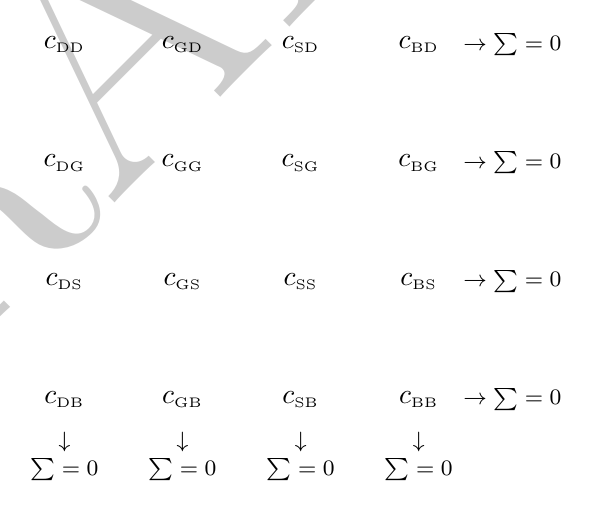
\begin{tikzpicture}[scale=0.75]
    \node[] at (-3,3) {$c_{{\scriptscriptstyle\mathrm{DD}}}$};
    \node[] at (-3,1) {$c_{{\scriptscriptstyle\mathrm{DG}}}$};
    \node[] at (-3,-1) {$c_{{\scriptscriptstyle\mathrm{DS}}}$};
    \node[] at (-3,-3) {$c_{{\scriptscriptstyle\mathrm{DB}}}$};
    \node[] at (-1,3) {$c_{{\scriptscriptstyle\mathrm{GD}}}$};
    \node[] at (-1,1) {$c_{{\scriptscriptstyle\mathrm{GG}}}$};
    \node[] at (-1,-1) {$c_{{\scriptscriptstyle\mathrm{GS}}}$};
    \node[] at (-1,-3) {$c_{{\scriptscriptstyle\mathrm{GB}}}$}; 
    \node[] at (1,3) {$c_{{\scriptscriptstyle\mathrm{SD}}}$};
    \node[] at (1,1) {$c_{{\scriptscriptstyle\mathrm{SG}}}$};
    \node[] at (1,-1) {$c_{{\scriptscriptstyle\mathrm{SS}}}$};
    \node[] at (1,-3) {$c_{{\scriptscriptstyle\mathrm{SB}}}$};  
    \node[] at (3,3) {$c_{{\scriptscriptstyle\mathrm{BD}}}$};
    \node[] at (3,1) {$c_{{\scriptscriptstyle\mathrm{BG}}}$};
    \node[] at (3,-1) {$c_{{\scriptscriptstyle\mathrm{BS}}}$};
    \node[] at (3,-3) {$c_{{\scriptscriptstyle\mathrm{BB}}}$};  
    
    \node[anchor=west,font=\footnotesize,inner sep=1pt] at (3.7,-3) {$\rightarrow \sum=0$}; 
    \node[anchor=west,font=\footnotesize,inner sep=1pt] at (3.7,-1) {$\rightarrow \sum=0$}; 
    \node[anchor=west,font=\footnotesize,inner sep=1pt] at (3.7,1) {$\rightarrow \sum=0$};  
    \node[anchor=west,font=\footnotesize,inner sep=1pt] at (3.7,3) {$\rightarrow \sum=0$};  
    
    \node[anchor=north,font=\footnotesize,inner sep=1pt] (a) at (-3,-3.5) {$\downarrow$}; 
    \node[anchor=north,font=\footnotesize,inner sep=1pt] (b) at (-1,-3.5) {$\downarrow$}; 
    \node[anchor=north,font=\footnotesize,inner sep=1pt] (c) at (1,-3.5) {$\downarrow$};  
    \node[anchor=north,font=\footnotesize,inner sep=1pt] (d) at (3,-3.5) {$\downarrow$};    
    
    \node[anchor=north,font=\footnotesize,inner sep=1pt] () at (a.south)  {$\sum=0$}; 
    \node[anchor=north,font=\footnotesize,inner sep=1pt] () at (b.south)  {$\sum=0$}; 
    \node[anchor=north,font=\footnotesize,inner sep=1pt] () at (c.south)  {$\sum=0$}; 
    \node[anchor=north,font=\footnotesize,inner sep=1pt] () at (d.south)  {$\sum=0$}; 
  \end{tikzpicture}
  \caption{Kapazitäten als Tabelle angeordnet}
  \label{fig:caps}
\end{figure}

\si{100.00}


\begin{table}[H]
\centering
\caption{Various operating points of }
\begin{tabular}{cccccccc}
\toprule
Property                                    & Unit                 &  ~         &  ~         &  ~         &     ~      &  ~         &     ~      \\ \midrule 
$V_{\mathrm{S}}$                            & \si{\milli\volt}     & \si{200.0} & \si{200.0} & \si{200.0} & \si{200.0} & \si{200.0} & \si{200.0} \\
$V_{\mathrm{B}}$                            & \si{\milli\volt}     & \si{100.0} & \si{100.0} & \si{100.0} & \si{100.0} & \si{100.0} & \si{100.0} \\
$V_{\mathrm{G}}$                            & \si{\milli\volt}     &  ~         &  ~         &  ~         &     ~      &  ~         &     ~      \\
$V_{\mathrm{D}}$                            & \si{\milli\volt}     &  ~         &  ~         &  ~         &     ~      &  ~         &     ~      \\ \midrule
$V_{\mathrm{GS}}$                           & \si{\volt}           &  ~         &  ~         &  ~         &     ~      &  ~         &     ~      \\
$V_{\mathrm{DS}}$                           & \si{\volt}           &  ~         &  ~         &  ~         &     ~      &  ~         &     ~      \\
$V_{\mathrm{GS,i}}$                         & \si{\volt}           &  ~         &  ~         &  ~         &     ~      &  ~         &     ~      \\
$V_{\mathrm{DS,i}}$                         & \si{\volt}           &  ~         &  ~         &  ~         &     ~      &  ~         &     ~      \\ \midrule
$V_{\mathrm{TH}}$                           & \si{\volt}           &  ~         &  ~         &  ~         &     ~      &  ~         &     ~      \\
$V_{\mathrm{OV}}$                           & \si{\volt}           & ~          &  ~         &  ~         &     ~      &  ~         &     ~      \\
$I_{\mathrm{D}}$                            & \si{\ampere}         &  ~         &  ~         &  ~         &     ~      &  ~         &     ~      \\
$I_{\mathrm{S}}$                            & \si{\ampere}         &  ~         &  ~         &  ~         &     ~      &  ~         &     ~      \\
$I_{\mathrm{G}}$                            & \si{\ampere}         &  ~         &  ~         &  ~         &     ~      &  ~         &     ~      \\
$I_{\mathrm{B}}$                            & \si{\ampere}         &  ~         &  ~         &  ~         &     ~      &  ~         &     ~      \\
$g_{\mathrm{m}}$                            & \si{\siemens}        &  ~         &  ~         &  ~         &     ~      &  ~         &     ~      \\
$\nicefrac{g_{\mathrm{m}}}{I_{\mathrm{D}}}$ & \si{\per\volt}       &  ~         &  ~         &  ~         &     ~      &  ~         &     ~      \\ \midrule
$Q_{\mathrm{B}}$                            & \si{\coulomb}        &  ~         &  ~         &  ~         &     ~      &  ~         &     ~      \\
$Q_{\mathrm{D}}$                            & \si{\coulomb}        &  ~         &  ~         &  ~         &     ~      &  ~         &     ~      \\
$Q_{\mathrm{S}}$                            & \si{\coulomb}        &  ~         &  ~         &  ~         &     ~      &  ~         &     ~      \\
$Q_{\mathrm{G}}$                            & \si{\coulomb}        &  ~         &  ~         &  ~         &     ~      &  ~         &     ~      \\ \midrule
$C_{\mathrm{DD}}$                           & \si{\farad}          &  ~         &  ~         &  ~         &     ~      &  ~         &     ~      \\
$C_{\mathrm{DG}}$                           & \si{\farad}          &  ~         &  ~         &  ~         &     ~      &  ~         &     ~      \\
$C_{\mathrm{DS}}$                           & \si{\farad}          &  ~         &  ~         &  ~         &     ~      &  ~         &     ~      \\
$C_{\mathrm{DB}}$                           & \si{\farad}          &  ~         &  ~         &  ~         &     ~      &  ~         &     ~      \\ 
$C_{\mathrm{GD}}$                           & \si{\farad}          &  ~         &  ~         &  ~         &     ~      &  ~         &     ~      \\
$C_{\mathrm{GG}}$                           & \si{\farad}          &  ~         &  ~         &  ~         &     ~      &  ~         &     ~      \\
$C_{\mathrm{GS}}$                           & \si{\farad}          &  ~         &  ~         &  ~         &     ~      &  ~         &     ~      \\
$C_{\mathrm{GB}}$                           & \si{\farad}          &  ~         &  ~         &  ~         &     ~      &  ~         &     ~      \\ 
$C_{\mathrm{SD}}$                           & \si{\farad}          &  ~         &  ~         &  ~         &     ~      &  ~         &     ~      \\
$C_{\mathrm{SG}}$                           & \si{\farad}          &  ~         &  ~         &  ~         &     ~      &  ~         &     ~      \\
$C_{\mathrm{SS}}$                           & \si{\farad}          &  ~         &  ~         &  ~         &     ~      &  ~         &     ~      \\
$C_{\mathrm{SB}}$                           & \si{\farad}          &  ~         &  ~         &  ~         &     ~      &  ~         &     ~      \\ 
$C_{\mathrm{BD}}$                           & \si{\farad}          &  ~         &  ~         &  ~         &     ~      &  ~         &     ~      \\
$C_{\mathrm{BG}}$                           & \si{\farad}          &  ~         &  ~         &  ~         &     ~      &  ~         &     ~      \\
$C_{\mathrm{BS}}$                           & \si{\farad}          &  ~         &  ~         &  ~         &     ~      &  ~         &     ~      \\
$C_{\mathrm{BB}}$                           & \si{\farad}          &  ~         &  ~         &  ~         &     ~      &  ~         &     ~      \\ \midrule 
\end{tabular}
\label{tab:regions}
\end{table}


\begin{align}\label{eq:bsim3v3-caps}
C_{\mathrm{GS}} &= - c_{{\scriptscriptstyle \mathrm{GS}}}  &  C_{\mathrm{DS}} &= - c_{{\scriptscriptstyle \mathrm{SD}}}  &  C_{\mathrm{m}}  &=  c_{{\scriptscriptstyle \mathrm{GD}}} - c_{{\scriptscriptstyle \mathrm{DG}}} \nonumber\\
C_{\mathrm{GD}} &= - c_{{\scriptscriptstyle \mathrm{GD}}}  &  C_{\mathrm{SB}} &= - c_{{\scriptscriptstyle \mathrm{BS}}}  &  C_{\mathrm{mb}} &=  c_{{\scriptscriptstyle \mathrm{BD}}} - c_{{\scriptscriptstyle \mathrm{DB}}} \\
C_{\mathrm{GB}} &= - c_{{\scriptscriptstyle \mathrm{GB}}}  &  C_{\mathrm{DB}} &= - c_{{\scriptscriptstyle \mathrm{BD}}}  &  C_{\mathrm{mx}} &=  c_{{\scriptscriptstyle \mathrm{GB}}} - c_{{\scriptscriptstyle \mathrm{BG}}} \nonumber
\end{align}


\printbibliography
\end{document}